
\chapter{Light Field Photography}

The propagation of the light rays in the 3D space can be completely described by a 7D continuous function $R(\theta,\phi,\lambda,\tau,V_x,V_y,V_z)$, where $(V_x,V_y,V_z)$ is a location in the 3D space, $(\theta,\phi)$ are propagation angles, $\lambda$ is the wavelength and $\tau$ the time; this function is known as the plenoptic function and describes the amount of light flowing in every direction through every point in space an any time, the magnitude of $R$ is known as the radiance.  In an 1846 lecture entitled "Thoughts on Ray Vibrations" Michael Faraday proposed for the first time that light could be interpreted as a field, inspired by his work on magnetic fields; but the idea of a plenoptic function representing the spectral radiance distribution of rays was first proposed by Adelson and Bergen \cite{Adelson-Plenoptic}. 

\bigskip

\begin{figure}[h!]
\centering
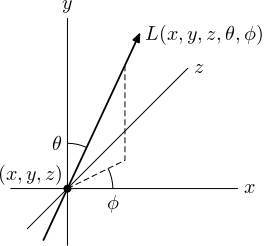
\includegraphics[width=0.5\textwidth]{./Diagrams/Plenoptic_function.jpg}
\caption{Spatio-angular parametrization of the plenoptic function for fixed $\tau$ and $\lambda$. Figure taken from Wikipedia (https://en.wikipedia.org/wiki/Light\_field)}
\end{figure}

\bigskip

In a more practical approach the plenoptic function can be simplified to a 4D version, called 4D Light Field or simply Light Field (abbreviated from now on as LF), denoted as the function $L$. The LF quantifies the intensity of static and monochromatic light rays propagating in half space, though this seems like an important reduction of information, this constraint does not substantially limit us in the accurate 3D description of the scene from where the light rays come from.

\bigskip 

 There exists three tipical forms of this 4D approximation: 
\begin{enumerate}
\item The LF rays positions are indexed by their Cartesian coordinates on two parallel planes, also called the two-plane parametrization $L(u,v,s,t)$.
\item The LF rays positions are indexed by their Cartesian coordinates on a plane and the directional angles leaving each point, $L(u,v,\phi,\theta)$.
\item Pairs of points on the surface of a sphere $L(\phi_1,\theta_1,\phi_2,\theta_2)$.
\end{enumerate}

\bigskip

\begin{figure}[h!]
\centering
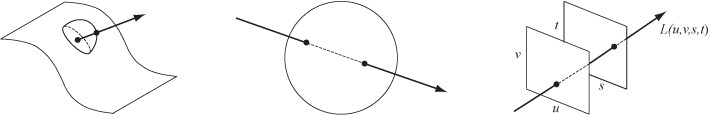
\includegraphics[width=1.0\textwidth]{./Diagrams/Light-field-parametrizations.jpg}
\caption{Three different representations of 4D LF\@. Left: $L(u,v,\phi,\theta)$. Center: $L(\phi_1,\theta_1,\phi_2,\theta_2)$. Right: $L(u,v,s,t)$. Figure taken from Wikipedia (https://en.wikipedia.org/wiki/Light\_field)}
\end{figure}

\bigskip

In this work we will centered our attention in the two plane parametrization $L(u,v,s,t)$, if you are interested in the other descriptions we recommend to see \cite{Liang}. In order to understand deeply this way of LF description, lets consider a camera with image plane coordinates $(u,v)$ and the focal distance $f$ moving along the $(s,t)$ plane. 

\bigskip

\begin{figure}[h!]
\centering
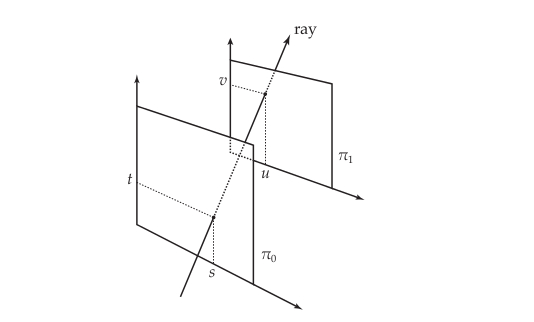
\includegraphics[width=1.0\textwidth]{./Diagrams/two-planes_param.jpg}
\caption{Graphic representation of the two plane parametrization of a single ray on the LF which is parametrized by the intersection $(s,t)$ and $(u,v)$ with planes $\pi_0$ and $\pi_1$, respectively. Figure taken from \cite{Kim-Disney} p.21}
\end{figure}

\bigskip

For simplicity one can constrain the vertical camera motion by fixing $s = s_0$ and moving the camera along the $t-axes$ in an straight light motion, in the section~\ref{sec:Epi-geometry} we will see that this constraint leads to an elegant geometric 3D representation of the scene called Epipolar Geometry, this multiview aquisition is refered as parallax only (HPO). Under this constraint, images captured by successive camera positions $t_1$, $t_2$,\ldots\ can be stacked together, and one can also interpret each camera position as a time step.

\bigskip

\begin{figure}[h!]
\centering
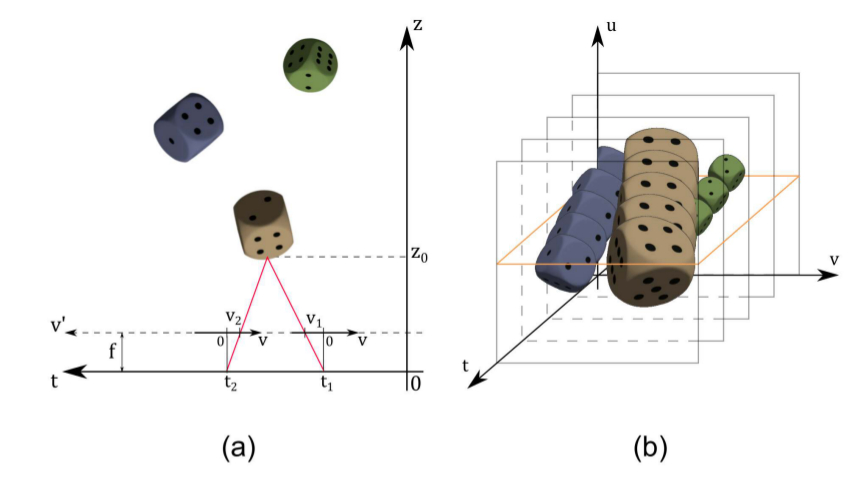
\includegraphics[width= 0.90\textwidth]{./Diagrams/images_stacked.jpg}
\caption{Stacked captured images represented in (b) from the scene setup (a). Figure taken from \cite{LF-Shearlets} p. 2}
\end{figure}

\section{Light Field Photography in the History}

For different reasons of interest for science and art capturing light fields has been an active research area for more than 110 years (the reason will be explained in detail on the section~\ref{sec:LF-applications}). In 1903 Herbert E. Ives \cite{Ives} was the first to realize that the light field inside a camera can be recorded by placing a pinhole or lenslet arrays in front of a film sensor (what is know as pinhole camera). On the other hand, in 1908 the french physicist and Nobel laureate Gabriel Lippmann published two articles about something that he called \textit{photographie int\'egrale} (translated as integral photography) \cite{Lippmann} in which he describes an imaging apparatus with an arrange of small lenses on a 2D grid that are able to capture multiple images of a scene with viewpoint variations; the captured scene is reproduced in 3D as the viewer sees the parallax while the viewpoint changes. Is quite surprising that almost 110 year ago he could have the idea that modern state of the art LF aquisition systems use nowadays. 

\bigskip

Even some experiments to aquire the Light Field of a static scene were already proposed since the beginning of the XX century, the first contribution on the mathematical formalization of the Light Field Theory were proposed in 1991, when Adelson and Bergen \cite{AdelsonBergen} found a way to systematically categorize the visual elements in \textit{early vision}, which in combination, form visual information in the world. Here by \textit{early vision} we mean the processes that are involved in the first steps of the visual cortex, namely, basic segmentation, shape detection, motion analysis between others (for further information about \textit{early vision} \cite{Tomasiearly} is highly recommended); sor this purpose Adelson and Bergen defined the \textit{plenoptic function} which was already discussed at the beginning of this Chapter. 

\bigskip

The history of Light Field Theory can be separated in the three main steps in the study of the Light Field: The acquisition, the processing (which include in the most of the cases a geometry proxy) and the rendering, which are closely related, vary in computational complexity and for which there exist plenty of different approaches; in this thesis we will center our study on the first two steps. 

\bigskip

It is also worth to mention that in the last decade two companies had manufactured Cameras that are able to capture the 4D Light Field, also known as plenoptic cameras; the first was Raytrix founded by the german computer scientists Vhristian Perwass and Lennart Wietzke that released their camera in 2010 mostly focused on industrial application on 3D reconstruction (one can see their paper \cite{Raytrix} for a good reference) rather than general consumers. Later in 2012 the american company Lytro came out with a plenoptic camera that was the first consumer light field camera for the general public, that has as a principal feature the possibility to do refocusing in the pictures taken by the camera (as a reference for this camera we recommend to read the Stanford Technical Report written by the CEO of the company Ren Ng \cite{Lytro}). Both companies produce cameras that capture the light field using an array of lenses, this and other LF acquisition setting will be discuss in the next section.

\bigskip

\begin{figure}[h!]
\centering
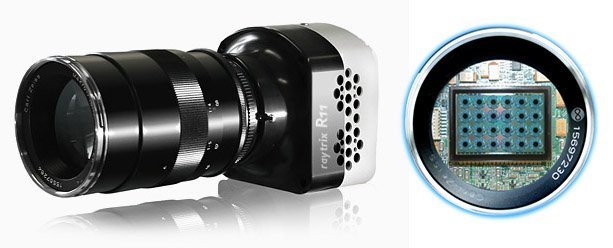
\includegraphics[width= 0.90\textwidth]{./Diagrams/raytrix.jpg}
\caption{Industrial plenoptic camera Raytrix R11, produced by Raytrix. Figure taken from \url{https://petapixel.com/assets/uploads/2010/09/raytrix.jpg}}
\end{figure}

\bigskip

\begin{figure}[h!]
\centering
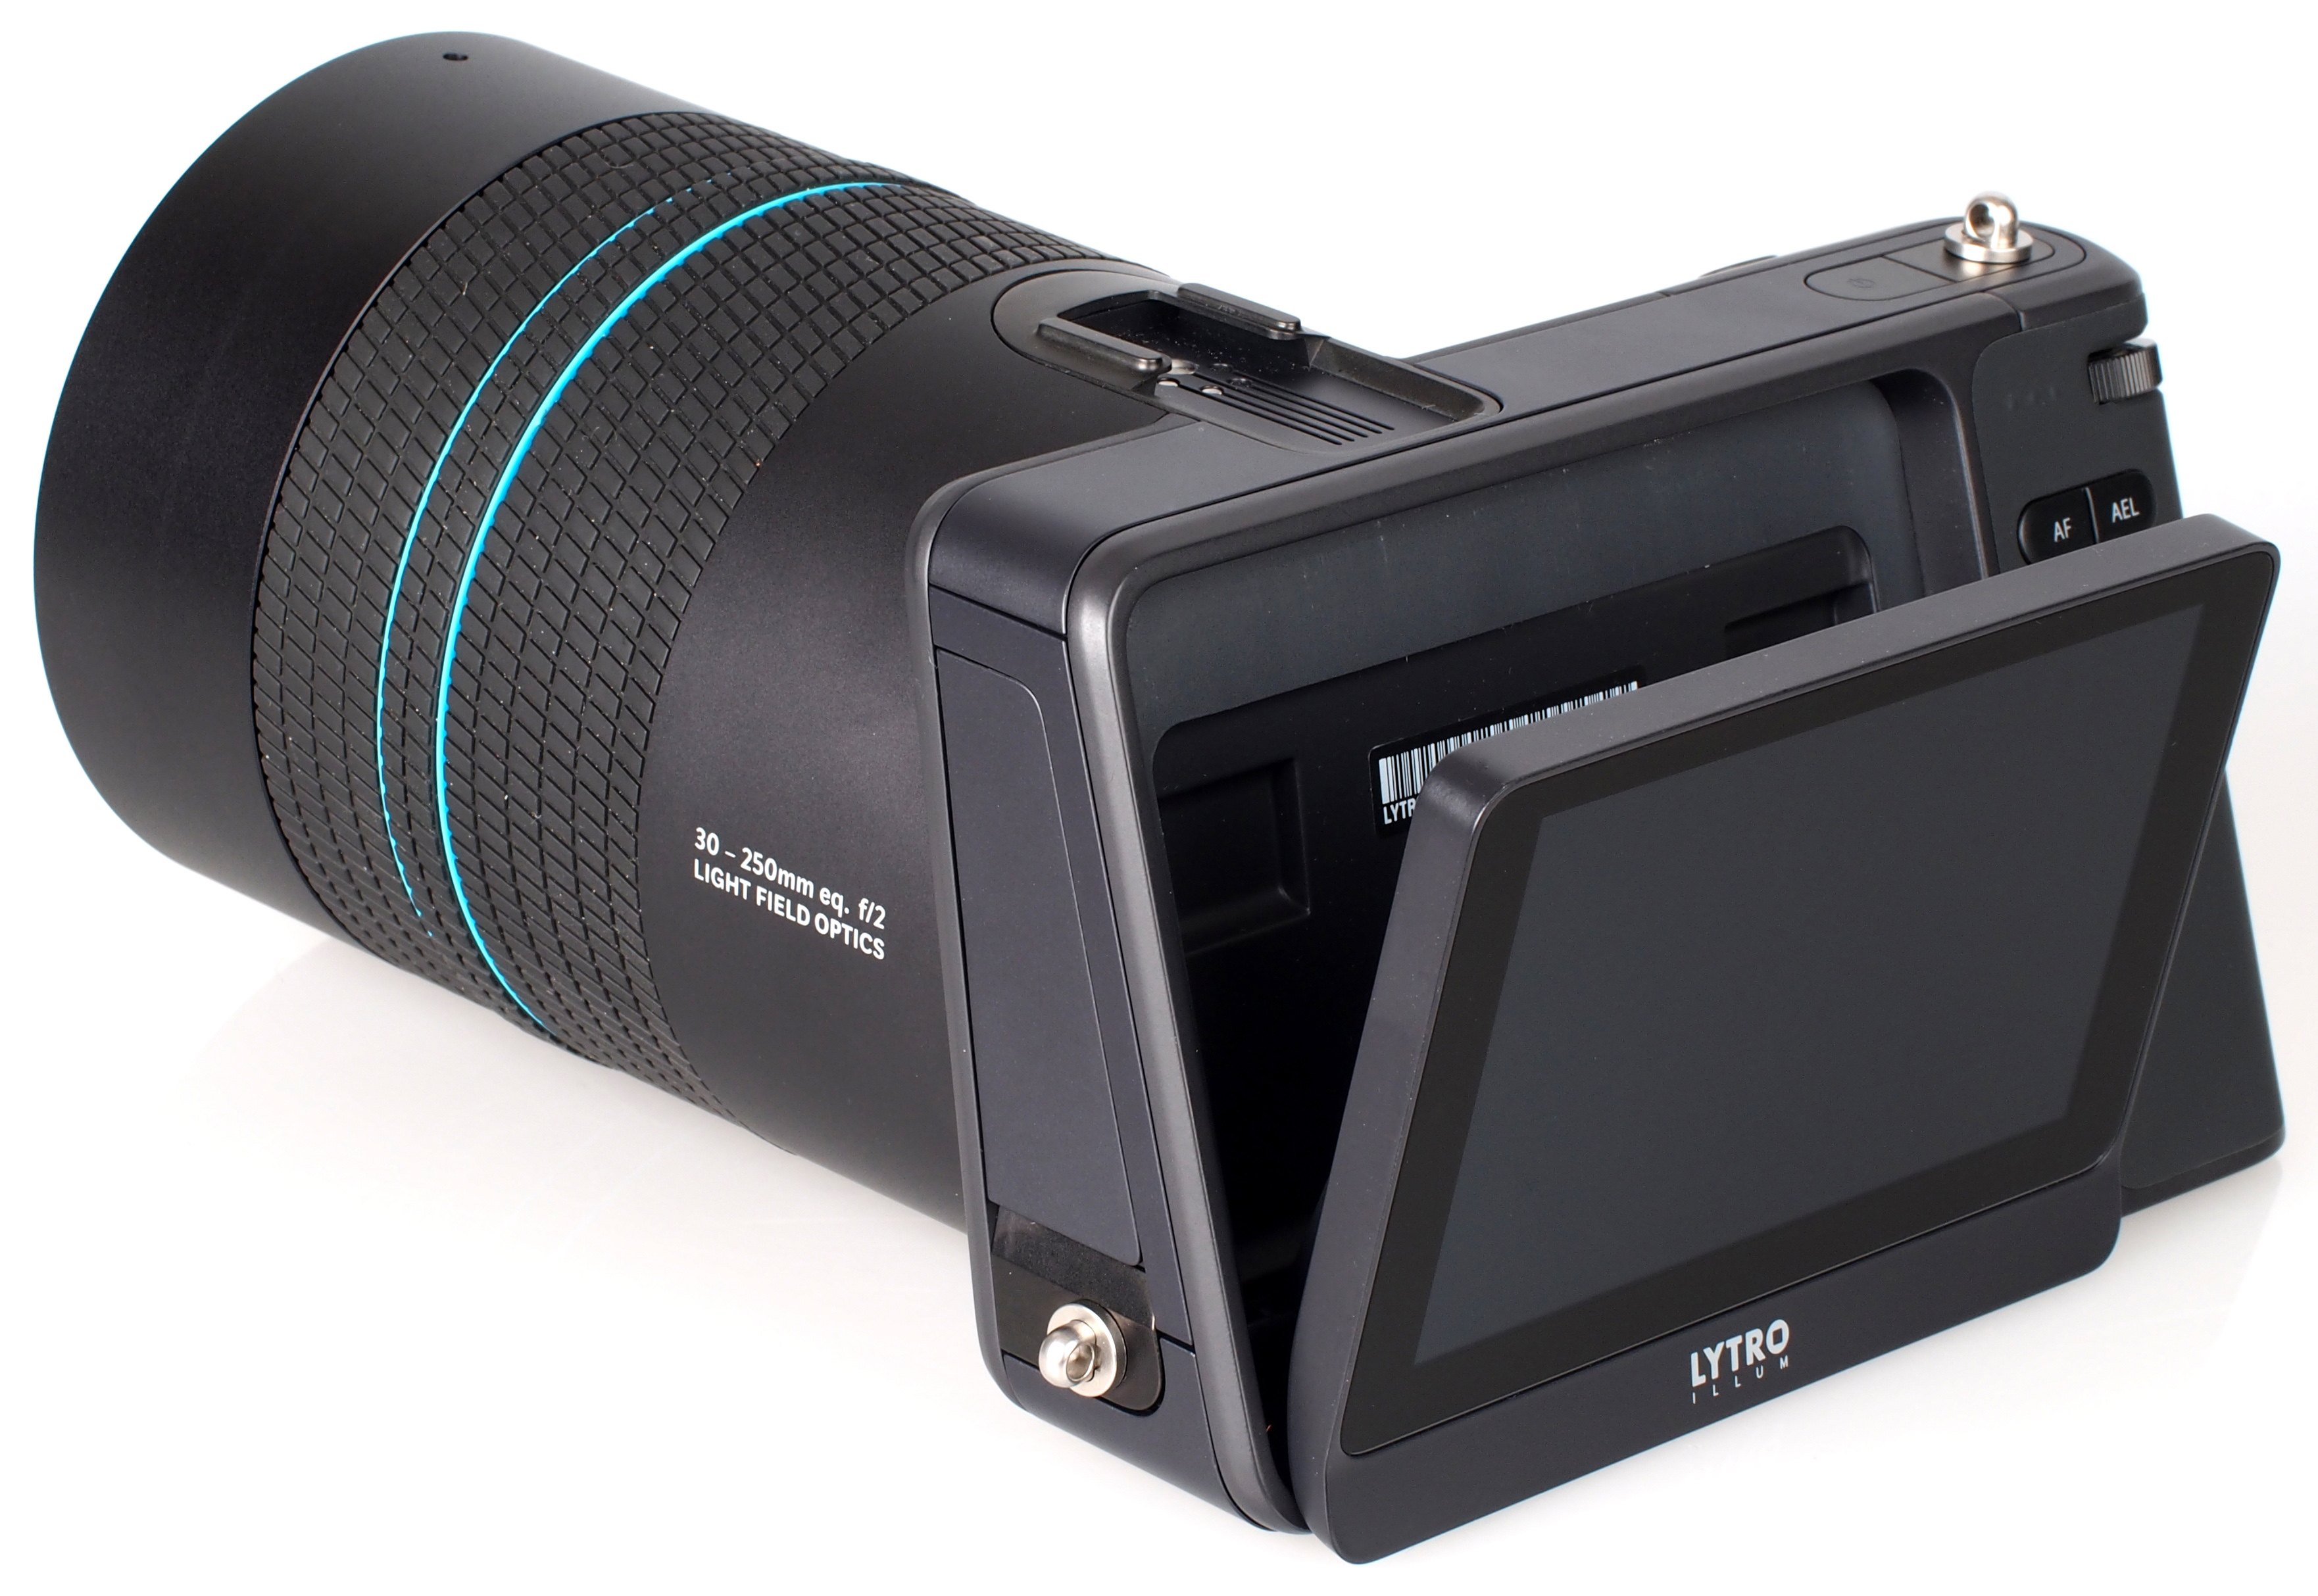
\includegraphics[width= 0.70\textwidth]{./Diagrams/lytro.jpg}
\caption{Consumer plenoptica camera Lytro Illum, produced by Lytro. Figure taken from \url{https://www.ephotozine.com/articles/lytro-illum-review-26434/images/highres-Lytro-Illum-6_1414410926.jpg}}
\end{figure}

\section{Light Field Acquisition Settings}
\label{sec:LF-acquisition}

The first creativity step in the experimental study of Light Field is the form of acquisition; using only our physical intuition is not trivial to come up with an idea of a system that captures faithfully the Light Field coming from a static scene that will be able to be processed by some straight-forward algorithm. From the beginning of the last century until today, scientists, engineers and hobbyists have proposed different approaches for the Light Field Acquisition Settings. 

\bigskip

As we have seen in the last section, the first attempts of settings were the pinhole camera proposed by Ives and the lenslet array proposed by Lippmann. The next variation of setting was proposed more than eighty years later by Adelson and Wang \cite{AdelsonWang} that in 1992 using the theory of plenoptic function (developed by Adelson itself) presented a design of a plenoptic camera where the light rays that pass through the main lens are recorded sparately using a lenticular array placed on the sensor plane, they used the light field recorded with this camera to obtain the scene depth by analyzing the directional variation of the radiance captured in the image; this is basically the Lippmann design but applied to digital cameras. Ng et al. \cite{Lytro} from Lytro used the same design of Adelson and Wang to produce the Lytro cameras.

\bigskip

\begin{figure}[h!]
\centering
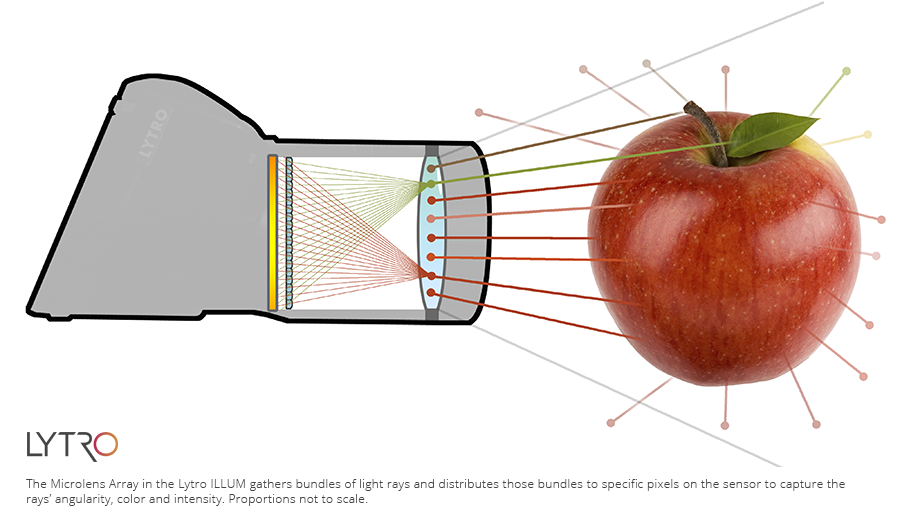
\includegraphics[width= 0.80\textwidth]{./Diagrams/lytro_array.png}
\caption{Diagram of Adelson and Wang design in Lytro cameras. Figure taken from \url{https://s3.amazonaws.com/lytro-corp-assets/blog/Lytro_ILLUM.png}}
\end{figure}

\bigskip

In 2006 Joshi et all \cite{Joshi} used a one-dimensional camera array and a motorized stage for for their real-time matting system. This technique of multicameras/multiviews acquisition is also quite common with camera arrays varying in position and size. The approach followed in this thesis take this technique as acquisition setting, the actual setup used will be explained in more detail in the section~\ref{sec:Sparse-acquisition}. The downside of this acquisition device is that in counterpart of the Lytro camera (hand-held) it can be built without having a priori a designed custom optics, but hey are bulky and often not portable (mechanical tracks are generally quite big and heavy).

\bigskip

A less bulky approach are the ones with Light-modulating codes in mask-based systems, that use coded masks in front of lenses for coded acquisition of the scene. Veeraraghavan et al. \cite{Veeraraghavan} where the first implementing a coded aperture technique to computatinally demultiplex the light rays collected through the camera's main lens. This attempt is less bulky than the multicameras and more light efficient than the pinhole arrays but it sacrifices image resolution, since the number of sensor pixels is the upper limit of the number of light rays captured (problem than camera arrays and lenslets does not have). To overcome this problem, Wetzstein et al. \cite{Wetzstein}, analized multiplexing light fields onto a 2D image sensor and developed a thoery for multiplexing and a computational reconstruction algorithm. 

\bigskip

A significant challenge of acquisition is that the captured set of images is very data-intensive and also redundant, mostly when one tries to recover high resolution light field form images with resolution above $(2000px)^2$. In order to tackle this issue, since the early papers on Light Field, the discussion about compact or sparse representation and compression schemes have played an important role in the area. For instance, Levoy and Hanrahan \cite{Levoy} proposed in 1995 several representations for 4D light fields and apply a lossy vector quantization followed by entropy coding; whereas Gortler et al. \cite{Gortler} in the same year applied standard image compression like JPEG to some of the views and pointed out the importance of depth information for sparser representation.

\bigskip

Later on Wetzstein with the Camera Culture Group of the MIT Media Lab developed a compressive light field camera architecture that allows for higher-resolution light fields to be recovered than previously possible from a single image, using three main components: light field atoms as a sparse representation of natural light fields (that involves dictionary learning which elements are the light field atoms), and optical design that allows for capturing optimized 2D light field projection also based in the coded masks technique, and robust sparse reconstruction methods to recover a 4D ligth field from a single coded 2D projection. In our opinion even this approach allows us to get a very high resolution of light fields, is a trade off by its requirements of high performance computation and its limitations coming from the baised learned dictionaries from a limited set of scenes. 

\bigskip

Due to the lack of equipment, 

\section{Typical applications for the Light Field Theory}
\label{sec:LF-applications}

\section{Geometric proxy: Stereo Vision and multiview Epipolar Geometry}
\label{sec:Epi-geometry}

\section{Physical and Computational Setup for Sparse acquisition of Epipolar-plane}
\label{sec:Sparse-acquisition}

